\documentclass[12pt, oneside, openany]{book}

%----------------------------------------------
% Encoding and Typography Enhancements
%----------------------------------------------
\usepackage[T1]{fontenc}            % Enhanced font encoding
\usepackage[utf8]{inputenc}         % Direct Unicode input
\usepackage{microtype}              % Fine-tune character spacing for better typography

%----------------------------------------------
% Primary and Mathematical Fonts
%----------------------------------------------
\usepackage{charter}                % Charter: legible serif for body text
\usepackage{mathpazo}               % Palatino-like math fonts
\usepackage{bm}                     % Bold math symbols

%----------------------------------------------
% Monospaced Font for Code Listings
%----------------------------------------------
\usepackage[scaled=.95]{inconsolata} % Inconsolata for code

%----------------------------------------------
% Page Layout and Spacing
%----------------------------------------------
\usepackage[a4paper, margin=1in]{geometry} % 1" margins on A4
\usepackage{setspace}              % Line-spacing control
\setstretch{1.3}                   % 1.3× line spacing

%----------------------------------------------
% Headers and Footers
%----------------------------------------------
\usepackage{fancyhdr}              % Fancy header/footer
\pagestyle{fancy}
\fancyhf{}
\fancyhead[L]{\nouppercase{\leftmark}} % Chapter title on left
\fancyhead[R]{\thepage}               % Page number on right
\fancypagestyle{plain}{               % Plain pages (e.g., chapter starts)
	\fancyhf{}
	\fancyfoot[C]{\thepage}
}

%----------------------------------------------
% Hyperlinks and PDF Metadata
%----------------------------------------------
\usepackage{hyperref}
\hypersetup{
	colorlinks    = true,
	linkcolor     = black,    % Internal links in black (print-friendly)
	citecolor     = blue,     % Citation links in blue
	urlcolor      = cyan,     % URLs in cyan
	pdfauthor     = {Mahdi},
	pdftitle      = {Arliz},
	pdfsubject    = {Programming, Arrays, and Data Structures},
	pdfkeywords   = {Arrays, Data Structures, Programming, History of Computing}
}

%----------------------------------------------
% Graphics and Diagrams
%----------------------------------------------
\usepackage{graphicx}             % Include images
\usepackage{caption}              % Customize captions
\usepackage{subcaption}           % Sub-figures support
\usepackage{xcolor}               % Color definitions
\usepackage{tikz}                 % Vector graphics & diagrams
\usetikzlibrary{positioning, shapes.geometric, arrows, calc}

%----------------------------------------------
% Tables and Arrays
%----------------------------------------------
\usepackage{array}                % Extended tabular features

%----------------------------------------------
% Section and Title Formatting
%----------------------------------------------
\usepackage{titlesec}             % Control title styles
\titleformat{\chapter}[display]
{\normalfont\huge\bfseries}{\chaptername\ \thechapter}{20pt}{\Huge}
\titleformat{\section}
{\Large\bfseries}{\thesection}{1em}{}
\titleformat{\subsection}
{\large\bfseries}{\thesubsection}{1em}{}

%----------------------------------------------
% Code Listings and Pseudocode
%----------------------------------------------
\usepackage{listings}             % Source code highlighting
\lstset{
	basicstyle      = \ttfamily\small,
	frame           = single,
	breaklines      = true,
	numbers         = left,
	numberstyle     = \tiny\color{gray},
	keywordstyle    = \color{myblue}\bfseries,
	commentstyle    = \color{olive},
	stringstyle     = \color{orange},
	backgroundcolor = \color{lightgray!20},
	captionpos      = b,
	escapeinside    = {(*@}{@*)},
	morekeywords    = {array, structure, algorithm, complexity}
}

\usepackage{algorithm}             % Algorithm floats
\usepackage{algpseudocode}         % Pseudocode environment

%----------------------------------------------
% Color Definitions
%----------------------------------------------
\definecolor{myblue}{RGB}{0, 102, 204}     % Custom blue for code
\definecolor{lightgray}{RGB}{240, 240, 240} % Light gray background

%----------------------------------------------
% Special Boxes and Environments
%----------------------------------------------
\usepackage{tcolorbox}
\tcbuselibrary{most}

\newtcolorbox{notebox}[1][]{
	colback   = blue!5!white,
	colframe  = blue!75!black,
	title     = Note,
	#1
}
\newtcolorbox{tipbox}[1][]{
	colback   = green!5!white,
	colframe  = green!75!black,
	title     = Tip,
	#1
}
\newtcolorbox{warningbox}[1][]{
	colback   = red!5!white,
	colframe  = red!75!black,
	title     = Important,
	#1
}

%----------------------------------------------
% Bibliography and Citations
%----------------------------------------------
\usepackage[backend=biber,style=apa]{biblatex}
\addbibresource{references.bib}

%----------------------------------------------
% Table of Contents, Bibliography, Index
%----------------------------------------------
\usepackage{tocbibind}            % Include TOC adds
\usepackage{imakeidx}             % Index creation
\makeindex

%----------------------------------------------
% Multiple Columns (e.g., Glossary)
%----------------------------------------------
\usepackage{multicol}

%----------------------------------------------
% PDF Inclusion (e.g., for front matter pages)
%----------------------------------------------
\usepackage{pdfpages}
\begin{document}
	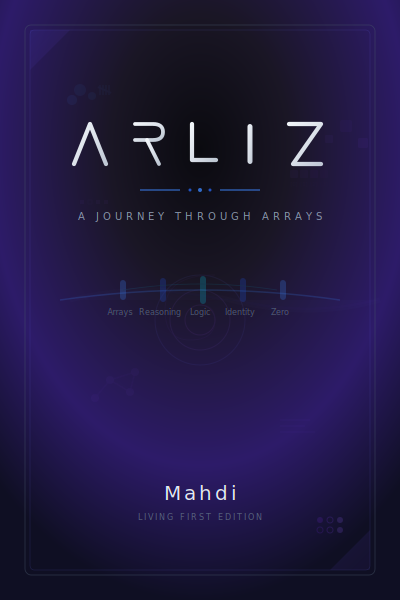
\includepdf[pages=-, pagecommand={\thispagestyle{empty}}, width=\paperwidth, height=\paperheight]{logo.pdf}
	
	\frontmatter
	% Title Page (Front Matter)

\begin{titlepage}
	\begin{center}
		\vspace*{2cm}

		{\Huge\bfseries In Praise of Arliz}\\[2em]
		
		{\Large\scshape Mahdi}\\[0.5em]
		
		\begin{minipage}{1\textwidth}
			\centering
			This book evolves. Every insight gained—whether a circuit, a structure,\\
				or a simple idea—is absorbed and integrated. 
		\end{minipage}
		
		\vfill
		
	{\large \textsc{First Edition}}\\[0.5em]
	{\large \today}
	
	\vspace*{1cm}
	{\small
		\textcopyright\ 2025 Mahdi “Genix”  
		\par
		Released under the MIT License  
	}
	\end{center}
\end{titlepage}

%----------------------------------------------
% Dedication
%----------------------------------------------
\thispagestyle{empty}
\vspace*{6cm}
\begin{center}
	\emph{
		To those who build from first principles.\\
		To the silent thinkers who design before they speak.\\
		To the ones who see in systems—\\
		not just machines, but metaphors.\\
		This is for you.}
\end{center}

\pagestyle{empty}
	\chapter{Preface}
	\thispagestyle{empty}

	%\maketitle
	Every book has its own story, and this book is no exception. If I were to summarize the process of creating this book in one word, that word would be “improvised.” Yet the truth is that Arliz is the result of pure, persistent curiosity that has grown in my mind for years. What you are reading now could be called a technical book, a collection of personal notes, or even a journal of unanswered questions and curiosities. But I—officially—call it a \emph{book}, because it is written not only for others but for myself, as a record of my learning journey and an effort to understand more precisely the concepts that once seemed obscure and, at times, frustrating.\\
	The story of Arliz began with a simple feeling: \textbf{curiosity}.  
	Curiosity about what an array truly is. Perhaps for many this question seems trivial, but for me this word—encountered again and again in algorithm and data structure discussions—always raised a persistent question.\\
	Every time I saw terms like \texttt{array}, \texttt{stack}, \texttt{queue}, \texttt{linked list}, \texttt{hash table}, or \texttt{heap}, I not only felt confused but sensed that something fundamental was missing. It was as if a key piece of the puzzle had been left out. The first brief, straightforward explanations I found in various sources never sufficed; they assumed you already knew exactly what an array is and why you should use it. But I was looking for the \emph{roots}. I wanted to understand from zero what an array means, how it was born, and what hidden capacities it holds.\\
	That realization led me to decide:  
	\emph{If I truly want to understand, I must start from zero.}\\	
	There is no deeper story behind the name “Arliz.” There is no hidden philosophy or special inspiration—just a random choice. I simply declared:  
	\emph{This book is called Arliz.}  
	You may pronounce it "Ar-liz," "Array-Liz," or any way you like. I personally say "ar-liz." That is all—simple and arbitrary.\\	
	But Arliz is not merely a technical book on data structures. In fact, \textbf{Arliz grows alongside me}. \\
	Whenever I learn something I deem worth writing, I add it to this book. Whenever I feel a section could be explained better or more precisely, I revise it. Whenever a new idea strikes me—an algorithm, an exercise, or even a simple diagram to clarify a structure—I incorporate it into Arliz.\\
	This means Arliz is a living project. As long as I keep learning, Arliz will remain alive.\\	
	The structure of this book has evolved around a simple belief: true understanding begins with context. That’s why Arliz doesn’t start with code or syntax, but with the origins of computation itself. We begin with the earliest tools and ideas—counting stones, the abacus, mechanical gears, and early notions of logic—long before transistors or binary digits came into play. From there, we follow the evolution of computing: from ancient methods of calculation to vacuum tubes and silicon chips, from Babbage’s Analytical Engine to the modern microprocessor. Along this journey, we discover that concepts like arrays aren’t recent inventions—they are the culmination of centuries of thought about how to structure, store, and process information.\\
	In writing this book, I have always tried to follow three principles:
	
	\begin{itemize}
		\item \textbf{Simplicity of Expression:} I strive to present concepts in the simplest form possible, so they are accessible to beginners and not superficial or tedious for experienced readers.
		\item \textbf{Concept Visualization:} I use diagrams, figures, and visual examples to explain ideas that are hard to imagine, because I believe visual understanding has great staying power.
		\item \textbf{Clear Code and Pseudocode:} Nearly every topic is accompanied by code that can be easily translated into major languages like C\texttt{++}, Java, or C\#, aiming for both clarity and practicality.
	\end{itemize}
	
	An important note: many of the algorithms in Arliz are implemented by myself. I did not copy them from elsewhere, nor are they necessarily the most optimized versions. My goal has been to understand and build them from scratch rather than memorize ready-made solutions. Therefore, some may run slower than standard implementations—or sometimes even faster. For me, the process of understanding and constructing has been more important than simply reaching the fastest result.\\	
	Finally, let me tell you a bit about myself:  
	I am \textbf{Mehdi}. If you prefer, you can call me by my alias: \emph{Genix}. I am a student of Computer Engineering (at least at the time of writing this). I grew up with computers—from simple games to typing commands in the terminal—and I have always wondered what lies behind this screen of black and green text. There is not much you need to know about me, just that I am someone who works with computers, sometimes gives them commands, and sometimes learns from them.\\	
	I hope this book will be useful for understanding concepts, beginning your learning journey, or diving deeper into data structures. \\	
	Arliz is freely available. You can access the PDF, LaTeX source, and related code at:  
	\begin{center}
		\url{https://github.com/m-mdy-m/Arliz}
	\end{center}
	In each chapter, I have included exercises and projects to aid your understanding. Please do not move on until you have completed these exercises, because true learning happens only by solving problems.\\	
	I hope this book serves you well—whether for starting out, reviewing, or simply satisfying your curiosity. And if you learn something, find an error, or have a suggestion, please let me know. As I said:
	\emph{This book grows with me.}
	
	% Acknowledgments
	\pagestyle{empty}
	\chapter{Acknowledgments}
		\thispagestyle{empty}
		I would like to express my gratitude to everyone who supported me during the creation of this book. Special thanks to the open-source community for their invaluable resources and to all those who reviewed early drafts and provided feedback.
		
		%\maketitle

	\tableofcontents
	\renewcommand{\arraystretch}{1.5} % Adjust row height for better readability
% Main Content
\mainmatter
\chapter*{How to Read This Book}

This book is not like most technical books you've probably encountered. It doesn't start with "Here's how to declare an array" or jump straight into syntax and algorithms. Instead, Arliz takes you on a journey—a long, winding path that begins thousands of years ago with humans counting on their fingers and ends with the sophisticated data structures we use today.\\
I know what you're thinking: "Why should I care about ancient history when I just want to learn arrays?" That's a fair question, and I've asked myself the same thing many times while writing this book. Here's the thing—understanding where something comes from changes how you think about it. When you know that arrays are not just programming constructs but the culmination of humanity's age-old quest to organize information, you start to see them differently. You begin to understand not just \emph{how} they work, but \emph{why} they work the way they do.\\
Arliz is structured in seven parts, each building upon the previous one:\\
\textbf{Part 1: Philosophical \& Historical Foundations} is where we are now. This part traces the human journey from basic counting to systematic representation. We explore ancient civilizations, their counting systems, the invention of the abacus, and the gradual development of mathematical thinking that made modern computation possible. This isn't just history for history's sake—it's the conceptual foundation that makes everything else make sense.\\
\textbf{Part 2: Mathematical Fundamentals} dives into the mathematical concepts that underlie all data structures. We cover set theory, functions, mathematical logic, and discrete mathematics. If Part 1 gives you the historical context, Part 2 gives you the mathematical tools to understand why data structures work the way they do.\\
\textbf{Part 3: Data Representation} explores how information is encoded in digital systems. We look at number systems, binary representation, character encoding, and the various ways computers store and manipulate data. This is where the abstract concepts from Parts 1 and 2 start to become concrete.\\
\textbf{Part 4: Computer Architecture \& Logic} examines the hardware foundations of computation. We explore logic gates, processor architecture, memory systems, and how the physical structure of computers influences the way we organize data.\\
\textbf{Part 5: Array Odyssey} is the heart of the book. Here, we finally meet arrays in all their glory—not as mysterious programming constructs, but as the natural evolution of thousands of years of human thought about organizing information. We explore their implementation, behavior, and applications in depth.\\
\textbf{Part 6: Data Structures \& Algorithms} expands beyond arrays to explore the broader landscape of data structures. Having understood arrays thoroughly, we can now appreciate how other structures like linked lists, trees, and graphs relate to and build upon array concepts.\\
\textbf{Part 7: Parallelism \& Systems} looks at how data structures behave in complex, multi-threaded, and distributed systems. This is where we explore the cutting edge of modern computation.\\
Now, you might be wondering: "Do I really need to read all of this? Can't I just skip to the arrays part?" \\
The honest answer is: it depends on who you are and what you want to get out of this book.\\
If you're a complete beginner—someone who's never programmed before, or who's just starting to learn about computer science—then yes, I strongly recommend reading the book from beginning to end. The concepts build upon each other in a way that's designed to create a solid, unshakeable foundation for your understanding.\\
If you're an experienced programmer who just wants to deepen your understanding of arrays specifically, you could potentially start with Part 5. However, I'd encourage you to at least skim Parts 1 and 2. You might be surprised by how much the historical and mathematical context enriches your understanding of concepts you thought you already knew.\\
If you're somewhere in between—maybe you know some programming but feel like you're missing fundamental concepts—then Parts 2, 3, and 4 might be your sweet spot. You can always come back to Part 1 later when you want to understand the bigger picture.\\
For students and educators, each part serves a different pedagogical purpose. Part 1 provides historical context and motivation. Parts 2-4 build theoretical foundations. Parts 5-7 provide practical application and advanced concepts. You can use different parts for different courses or learning objectives.\\
But here's what I really want you to understand: this book is not just about consuming information. It's about building intuition. Each part includes exercises, thought experiments, and projects designed to help you internalize the concepts. Don't skip these. They're not just busy work—they're carefully designed to help you develop the kind of deep, intuitive understanding that will serve you throughout your career.\\
One more thing: as I mentioned in the preface, this book grows with me. If you find errors, have suggestions, or discover better ways to explain something, please let me know. This is a living document, and your feedback helps make it better for everyone.\\
So, whether you're here for the full journey or just part of it, welcome to Arliz. Let's explore the fascinating world of arrays together—starting from the very beginning.\\


\part{Philosophical \& Historical Foundations}

\section*{Introduction}

Long before arrays existed as data structures in programming languages—long before computers, algorithms, or even formal mathematics—humans possessed an innate drive to organize, count, and systematically represent the world around them. This part of our journey explores not just the technical evolution of computational tools, but the profound intellectual transformation of human thought about order, sequence, and structured information.\\
Arrays are not merely programming constructs. They are the culmination of humanity's oldest and most fundamental intellectual pursuit: the systematic organization of information. Their conceptual roots stretch back thousands of years, embedded in the clay tablets of Mesopotamia, the geometric patterns of ancient Egypt, the bead arrangements of the abacus, and the philosophical frameworks of classical mathematics. To truly understand arrays, we must first understand the human mind's relentless quest to impose order upon chaos, to find patterns within complexity, and to create systems that can capture, manipulate, and transform structured knowledge.\\
Our exploration begins in the prehistoric dawn of human consciousness, when our ancestors first felt compelled to count beyond their fingers, to track seasons and harvests, to record transactions and astronomical observations. We witness the birth of positional notation in ancient Mesopotamia—the revolutionary idea that the \textbf{position} of a symbol could carry meaning, laying the conceptual groundwork for array indexing. We follow the development of the abacus across civilizations, seeing how different cultures refined this early computational array, creating sophisticated systems for parallel calculation that echo modern array operations.\\
As we progress through classical antiquity, we encounter the Greek philosophers who first formalized concepts of \textbf{sets}, \textbf{sequences}, and \textbf{ordered arrangements}. Aristotle's categorical thinking, Euclid's systematic geometry, and the Pythagorean exploration of number patterns all contributed essential building blocks for understanding structured data. The Chinese mathematical tradition, with its matrix-like arrangements for solving systems of equations, demonstrates early intuitive grasp of multidimensional data organization.\\
The medieval period brings us algorithmic thinking—Al-Khwarizmi's systematic procedures, the revolutionary introduction of zero and positional notation from the Hindu-Arabic tradition, and the monastic scriptoriums that pioneered systematic knowledge organization. These developments mark the transition from intuitive arrangement to formal, reproducible methods of data manipulation.\\
The Renaissance and early modern period witness the birth of symbolic thinking—Viète's algebraic notation, Descartes' coordinate systems, Pascal's triangular arrangements of combinatorial coefficients. Each breakthrough represents a step toward the abstract, systematic representation that enables modern computational thinking. By the time we reach the threshold of mechanical computation with Pascal's calculator and Leibniz's universal symbolic aspirations, the conceptual foundations for array-based thinking are fully established.\\
This historical foundation is not mere academic curiosity. Every concept explored in later parts of this book—from basic array operations to complex algorithmic optimizations—builds upon intellectual frameworks developed across millennia. Understanding this deep history provides not just context, but genuine insight into why arrays work the way they do, why certain operations are natural while others are complex, and how the fundamental patterns of structured thinking manifest in modern computational systems.\\
When you encounter array indexing, you're participating in a tradition that began with Mesopotamian scribes arranging cuneiform symbols on clay tablets. When you manipulate matrices, you're extending methods pioneered by Chinese mathematicians over two thousand years ago. When you design data structures, you're continuing humanity's ancient quest to create order from complexity, to find systematic methods for representing and transforming information.\\
This part prepares you for the mathematical formalism of Part 2, the technical implementation details of later sections, and ultimately, for a deeper appreciation of arrays as both practical tools and profound expressions of human intellectual achievement.
\newpage
\section*{How to Read}

This part is structured as a chronological journey through humanity's development of systematic thinking about information organization. Each chapter builds upon previous concepts while introducing new layers of complexity. The progression is intentionally gradual—from concrete counting methods to abstract mathematical frameworks—mirroring how human understanding evolved over millennia.\\
\textbf{For the Complete Journey:} Read chapters sequentially. This provides the full historical and conceptual foundation, showing how each civilization and era contributed essential elements to our modern understanding of structured data. Pay particular attention to recurring themes: position and place-value systems, systematic arrangement methods, symbolic representation, and the gradual abstraction from concrete tools to mathematical concepts.\\
\textbf{For Focused Study:} If you're primarily interested in specific aspects, you can emphasize certain chapters while skimming others.\\
\textbf{Connecting to Later Parts:} As you read, note how concepts introduced here reappear in mathematical formalization (Part 2), data representation (Part 3), and implementation details (Parts 4-7). The philosophical frameworks developed in early chapters provide context for technical decisions made in modern computing systems.\\
Each chapter includes timeline markers and focuses on specific conceptual developments. Don't merely read for historical facts—engage with the underlying ideas. Ask yourself: How did this development change how humans thought about organized information? What limitations did it overcome? What new possibilities did it create? This active engagement will deepen your understanding of both historical development and modern applications.

% ==========================================
% CHAPTER 1: THE PRIMORDIAL URGE TO COUNT AND ORDER
% ==========================================

\chapter{The Primordial Urge to Count and Order}
% Timeline: Pre-3500 BCE to 1000 BCE
% Focus: Basic human cognitive needs that led to structured thinking

\section{The Philosophy of Measurement and Representation}
% Why humans needed to count, measure, track - cognitive foundations

\section{From Stones to Symbols: Early Counting Systems}
% Tally marks, stone arrangements, body parts counting

\section{The Birth of Position and Place}
% Mesopotamian place-value systems, early positional notation

\section{Sacred Geometry and Ordered Patterns}
% Egyptian and Mesopotamian geometric arrangements, early pattern recognition

% ==========================================
% CHAPTER 2: ANCIENT CIVILIZATIONS AND SYSTEMATIC THINKING
% ==========================================

\chapter{Ancient Civilizations and Systematic Thinking}
% Timeline: 3500 BCE to 500 BCE
% Focus: Development of systematic approaches to knowledge organization

\section{Mesopotamian Clay Tablets and Cuneiform Arrays}
% Babylonian mathematical tablets, systematic arrangement of knowledge

\section{Egyptian Hieroglyphic Systems and Papyrus Records}
% Systematic record-keeping, inventory management, architectural planning

\section{Chinese Oracle Bones and Early Matrix Concepts}
% I-Ching arrangements, early binary-like thinking, systematic divination

\section{Indus Valley: Lost Systems of Organization}
% Archaeological evidence of systematic urban planning and notation

% ==========================================
% CHAPTER 3: THE ABACUS REVOLUTION
% ==========================================

\chapter{The Abacus Revolution: Humanity's First Computational Array}
% Timeline: 2700 BCE to 100 CE
% Focus: The abacus as the first true array-like computational tool

\section{Mesopotamian Counting Boards: The Genesis}
% Earliest dust abacus, groove-based calculations

\section{Chinese Suanpan: Perfecting the Art}
% Sophisticated bead arrangements, advanced calculations

\section{Greco-Roman Abacus: Spreading the Concept}
% Cultural transmission, adaptation to different number systems

\section{Philosophical Implications: State, Position, and Transformation}
% How the abacus embodies fundamental computational concepts

% ==========================================
% CHAPTER 4: CLASSICAL MATHEMATICAL FOUNDATIONS
% ==========================================

\chapter{Classical Mathematical Foundations}
% Timeline: 600 BCE to 400 CE
% Focus: Formal mathematical thinking that underlies array concepts

\section{Greek Philosophy of Numbers and Sets}
% Pythagorean number theory, Euclidean elements, concept of infinity

\section{Aristotelian Logic and Categorical Thinking}
% Categories, classifications, logical structures

\section{Diophantine Equations and Early Matrix Operations}
% Systems of equations, coefficient arrangements

\section{Chinese Mathematical Texts: The Nine Chapters}
% Systematic problem-solving, matrix-like coefficient arrangements

% ==========================================
% CHAPTER 5: MEDIEVAL SYNTHESIS AND THE ALGORITHMIC AWAKENING
% ==========================================

\chapter{Medieval Synthesis and the Algorithmic Awakening}
% Timeline: 500 CE to 1000 CE
% Focus: Integration of knowledge systems and birth of algorithmic thinking

\section{Islamic Golden Age: Al-Khwarizmi and Systematic Procedures}
% First algorithms, step-by-step procedures, algebraic thinking

\section{The Hindu-Arabic Numeral Revolution}
% Introduction of zero, positional notation impact on data organization

\section{Monastic Scriptoriums: Knowledge Preservation and Organization}
% Systematic cataloging, manuscript arrangement, early databases

\section{Persian and Central Asian Mathematical Traditions}
% Omar Khayyam's geometric algebra, systematic solution methods

% ==========================================
% CHAPTER 6: HIGH MEDIEVAL MATHEMATICAL RENAISSANCE
% ==========================================

\chapter{High Medieval Mathematical Renaissance}
% Timeline: 1000 CE to 1300 CE
% Focus: Formalization of mathematical thinking in medieval universities

\section{European University System: Systematic Mathematical Education}
% Quadrivium, systematic curriculum, formal mathematical training

\section{Fibonacci and the Liber Abaci: Bringing Systems to Europe}
% Systematic mathematical exposition, practical calculation methods

\section{Islamic Mathematical Synthesis: Al-Samaw'al and Polynomial Arrays}
% Systematic polynomial manipulation, coefficient arrangements

\section{Medieval Astronomy: Tabular Data and Systematic Observation}
% Astronomical tables, systematic data collection and arrangement

% ==========================================
% CHAPTER 7: LATE MEDIEVAL TO RENAISSANCE TRANSITION
% ==========================================

\chapter{Late Medieval to Renaissance Transition}
% Timeline: 1300 CE to 1500 CE
% Focus: Preparing the conceptual ground for systematic symbolic manipulation

\section{Scholastic Method: Systematic Logical Analysis}
% Systematic argumentation, logical structures, categorical thinking

\section{Commercial Mathematics: Practical Systematic Calculations}
% Merchant handbooks, systematic bookkeeping, tabular arrangements

\section{Medieval Islamic Algebraic Traditions}
% Systematic solution methods, algebraic symbolism development

\section{Early Renaissance Humanism: Rediscovery and Systematization}
% Recovery of classical texts, systematic comparison and analysis

% ==========================================
% CHAPTER 8: RENAISSANCE SYMBOLIC REVOLUTION
% ==========================================

\chapter{Renaissance Symbolic Revolution}
% Timeline: 1400 CE to 1600 CE
% Focus: Development of symbolic thinking that enables abstract array concepts

\section{Viète's Algebraic Symbolism: The Birth of Abstract Representation}
% Symbolic algebra, general methods, abstract mathematical thinking

\section{Cardano and Systematic Solution Methods}
% Cubic equations, systematic classification of solution types

\section{Decimal System Standardization: Stevin and Systematic Notation}
% Decimal fractions, systematic positional notation

\section{Renaissance Art and Mathematical Perspective: Systematic Spatial Representation}
% Linear perspective, systematic spatial arrangement, coordinate thinking

% ==========================================
% CHAPTER 9: EARLY MODERN MATHEMATICAL SYSTEMATIZATION
% ==========================================

\chapter{Early Modern Mathematical Systematization}
% Timeline: 1600 CE to 1700 CE
% Focus: Formal mathematical systems that directly enable array thinking

\section{Cartesian Coordinate System: Systematic Spatial Representation}
% Coordinate geometry, systematic position notation

\section{Leibniz's Characteristica Universalis: Dreams of Universal Symbolism}
% Universal symbolic language, systematic representation of thought

\section{Pascal's Triangle and Combinatorial Arrays}
% Systematic arrangement of combinatorial coefficients

\section{Early Probability Theory: Systematic Analysis of Uncertainty}
% Systematic enumeration, probabilistic thinking, tabular arrangements

% ==========================================
% CHAPTER 10: THE THRESHOLD OF MECHANICAL COMPUTATION
% ==========================================

\chapter{The Threshold of Mechanical Computation}
% Timeline: 1640 CE to 1800 CE
% Focus: Final conceptual steps before mechanical implementation

\section{Pascal's Calculator: Mechanizing Systematic Calculation}
% First mechanical calculator, systematic arithmetic operations

\section{Leibniz's Step Reckoner: Toward Universal Calculation}
% Mechanical multiplication, binary number system concepts

\section{Euler's Systematic Mathematical Notation}
% Function notation, systematic symbolic representation

\section{The Encyclopédie: Systematic Organization of Human Knowledge}
% Systematic classification, comprehensive knowledge organization

\part{Mathematical Fundamentals}
\section*{Introduction}
\section*{How to Read}
\part{Data Representation}
\section*{Introduction}
\section*{How to Read}
\part{Computer Architecture \& Logic}
\section*{Introduction}
\section*{How to Read}
\part{Array Odyssey}
\section*{Introduction}
\section*{How to Read}
\part{Data Structures \& Algorithms}
\section*{Introduction}
\section*{How to Read}
\part{Parallelism \& Systems}
\section*{Introduction}
\section*{How to Read}
\part{Synthesis \& Frontiers}
\section*{Introduction}
\section*{How to Read}
\end{document}